\documentclass[a4paper,11pt,english]{article}
\usepackage[english]{babel} 
\usepackage[T1]{fontenc}    
\usepackage[utf8]{inputenc} 
\usepackage{graphicx}       
\usepackage{hyperref}      


\begin{document}

\title{Active strategies for object discovery}
\author{Phil Bradfield \and Jan Fabian Schmid}
	
\maketitle 

\section{Introduction}
%Introduction, which describes the motivation and goal of your project. Describe how your project is connected to existing literature. Include references to scientific papers that are relevant to your topic. Do not copy your text from the intermediate report. Revise and rewrite according to the feedback you got and what the actual outcome of the project was.

In this final report of our project, we want to present our system, how it works, how it changed during the development, and how it performs.
The goal we had for our project was to develop an autonomous robot that is able to find areas corresponding to objects in its environment.
For autonomous systems in the future it is desirable that they are able to solve everyday life tasks of humans.
Since almost every meaningful everyday life task of humans contains interaction with at least some object of the environment, it is important that robots are able to find and use objects.
One of the first steps for this is object detection, which allows the robot to filter out relevant parts of its environment which are likely to correspond to an actual object. Having a model of nearby object positions and shapes could then allow the robot to go through this internal list and search for an object that might help him for his current task.
When a robot is visiting a place for the first time it might be a good idea to explore this room to create such a list of available objects.
This is the situation and the task that we want to solve with our system.
To be able to do this, it is necessary to perform simultaneous localization and mapping, detect potential objects in the current view, and to compute the next best view which allows to explore the environment.

\subsection{Related work}
Some existing approaches in the subject of object detection in autonomous robots are the following:

\section{Theoretical background}
%Theoretical background, which provides the descriptions on what existing theories and ideas that are related to your problem statement. The purpose of this section is to ensure that you are knowledgeable about the related key concepts, theories and models. Do not copy your text from the intermediate report. Revise and rewrite according to the feedback you got and what the actual outcome of the project was.

In this section we present some of the concepts and methods that we utilize in our system.

\subsection{Saliency-based object discovery}
To find objects in the robots current view, we use a saliency-based object discovery system.
Such a system has been introduced by García et al. \cite{garcia2015saliency}.
An overview of the method can be seen in Figure \ref{fig:2Dobject_discovery}.

\begin{figure}[h!]
	\begin{center}
		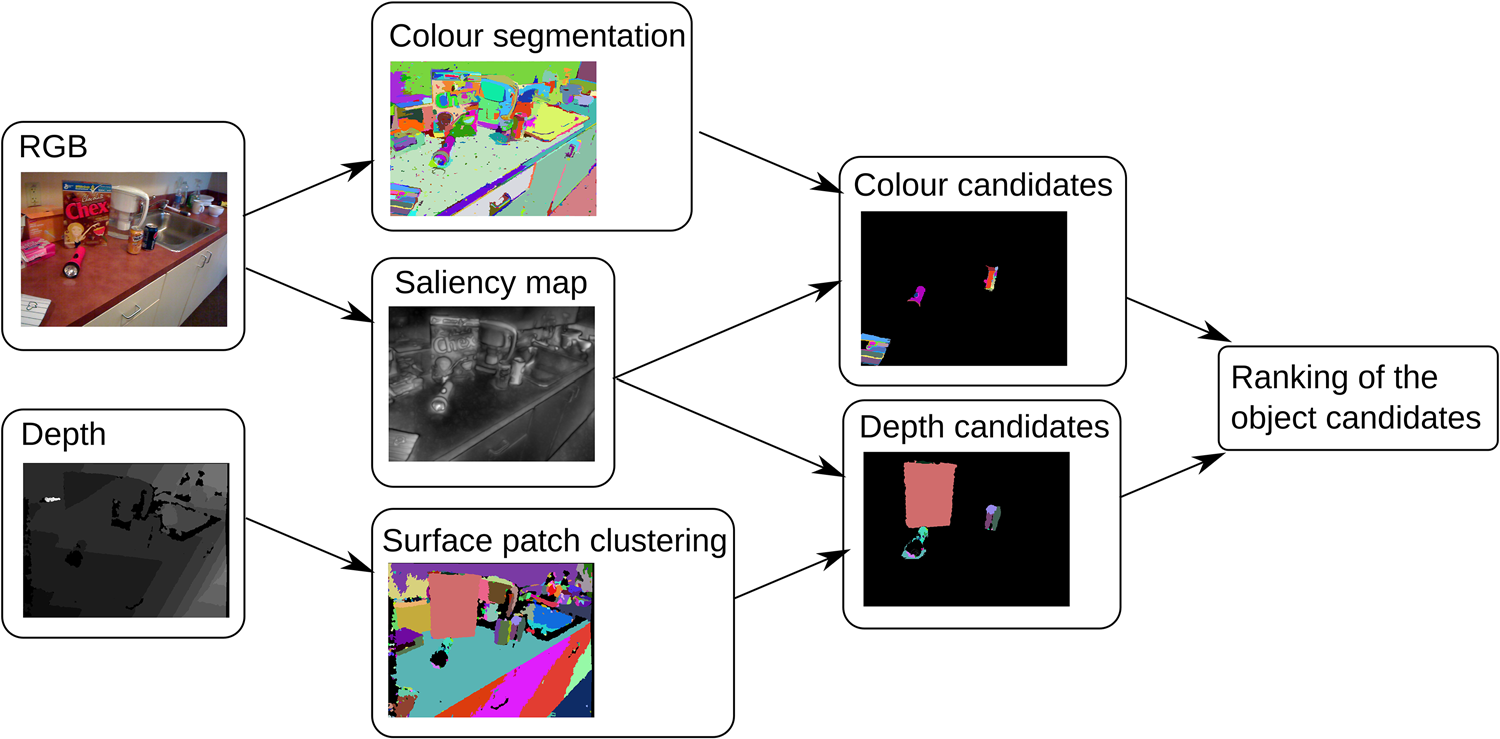
\includegraphics[width=1\textwidth]{src/saliency_object_detection.png}
		\caption{ Overview of the object candidate generation process \cite{garcia2015saliency}}
		\label{fig:2Dobject_discovery}
	\end{center}
\end{figure}

The method requires a colour and depth image of the same scene.
While it would work with colour information only experiments of the authors have shown that the combination of both achieves the best results.
The colour image is processed in two different ways: 
Using the Felzenszwalb and Huttenlocher algorithm \cite{felzenszwalb2004efficient} the image is segmented into small patches of similar colour.
Simultaneously a saliency map is computed. This is done with the VOCUS2 system developed by Frintrop et al. \cite{frintrop2015traditional}.
The general idea of VOCUS2 is to compute for each pixel a value quantifying its contrast to its proximate image area.
To generate object candidates the information of saliency map and colour segmentation are used together.
Seeded region growing is performed on the local maxima in the saliency map.
This means that starting from a local maxima neighboring pixels are iteratively grouped together into one region if their saliency value exceeds a certain percentage of the saliency value of the local maximum.
The result is a list of salient blobs in the saliency map.
For each salient blob one colour object candidate is created. It contains the pixels of all colour segments that overlap to at least $30\%$ with the pixels of the salient blob.
The depth candidates are generated analogous to the colour candidates, using the same salient blobs as a basis for the object candidates, but a surface clustering method is used as segmentation algorithm. It divides the image into continuous planes.
Afterwards, colour and depth candidates are merged into one set a ranking of proposed object candidates in terms of \glqq{}objectiveness\grqq{} takes place.

\subsection{Frontier exploration}
\subsection{Sampling-based exploration}
\subsection{Particle filter SLAM}
\subsection{Euclidean point cloud clustering}
\subsection{IoR mechanism to guide attention}
\subsection{Building a 3D map with octomap data structure}

\section{Implementation}
%Implementation, which connects with the section on theoretical background and describes how the required parts were implemented, and how the overall system is constructed.

\subsection{Overview of the system}
\begin{itemize}
	\item our hardware
	\item flowchart
\end{itemize}

\subsection{SLAM}
\begin{itemize}
	\item input: point cloud to laser scan and odometry from robot
	\item gmapping
	\item output: estimate of robot pose and 2d occupancy grid map
\end{itemize}

\subsection{Generation of object proposals}

\begin{itemize}
	\item 2D Object candidate generation
	\item Building the proposal point cloud
	\item Clustering the point cloud
	\item Projection of point cloud into map
	\item merging and handling of candidates in octomap
\end{itemize}

\subsection{NBV planning}

\begin{itemize}
	\item random
	\item frontier exploration
	\item information gain
	\begin{itemize}
	\item using the octomap
	\item IoR mechanism for obstacles
	\end{itemize}
\end{itemize}

\subsection{Robot navigation}

\section{Analysis}
% Results, which contain the descriptions of the experiments conducted and presents their results.

\subsection{Experimental setups}
\subsection{Metrics}
\subsection{Results}

\section{Conclusion}
%Conclusions, which summarizes the work that was done and the results obtained, and gives suggestions for future work. \textbf{Most importantly}, include a section that contrasts the actual outcome of the project to the plan you submitted: what was planned, what was actually achieved, what were the main reasons for the actual outcome, what you consider you have learned during the project, etc.

\subsection{Summary}
\subsection{Learnings and deviations from our original plans}
\subsection{Future work}

\newpage
\bibliographystyle{plain}
\addcontentsline{toc}{section}{Bibliography}% Add to the TOC
\bibliography{bib}

\end{document}
